%!TEX root = ./thesis-main.tex
\chapter{Analisi}

\section{Analisi dei requisiti}
Lo scopo principale del progetto è la realizzazione di una interfaccia web (quindi interpretabile da un qualsiasi browser moderno) che permetta l'interazione con il sistema software di simulazione
Alchemist in modo intuitivo e \textit{user-friendly}. Il compito dell'applicativo sarà quindi quello di comunicare, attraverso apposite \ac{API}, con l'infrastruttura server GraphQL preesistente e presentare, in seguito a cambiamenti nella simulazione o a richieste da parte dell'utente, un'interfaccia grafica che ne rappresenti i risultati.
\subsection{Requisiti funzionali}
\begin{itemize}
	\item L'applicativo dovrà presentare un' interfaccia grafica all'interno di un web browser.
	\item In una tipica simulazione di Alchemist sono presenti dei nodi. L'applicativo quindi dovrà essere in grado di rappresentare in un piano bidimensionale la posizione di tali nodi all'interno di un contesto grafico. Ciò implica ovviamente che con l'evolversi della simulazione il contesto grafico debba essere aggiornato. \footnote{Date le diverse \textit{incarnation} e i diversi possibili scenari che Alchemist può modellare non è detto che i nodi cambino di posizione.}
	\item Ogni nodo contiene diverse proprietà, reazioni, concentrazioni etc. L'interfaccia dovrà permettere di ispezionare il contenuto di ciascun nodo. 
	\item L'interfaccia dovrà controllare lo stato attuale della simulazione. Ciò vuol dire poterla eseguire o mettere in pausa.
\end{itemize}

\subsection{Requisiti non funzionali}
\begin{itemize}
	\item Interagendo con l'interfaccia, non si devono verificare tempi di risposta eccessivi. Per esempio se l'utente decide di ispezionare un nodo, il recupero di tali informazioni deve essere presentato in tempi ragionevoli.
	\item L'applicativo deve essere compatibile con un ambiente multipiattaforma.
	\item L'architettura delle componenti grafiche deve essere estendibile e facilmente modificabile.
\end{itemize}

\section{Requisiti implementativi}
Per la realizzazione di questo progetto, è stato necessario tener conto di due requisiti implementativi, tra cui l'uso di KotlinJS come linguaggio di sviluppo e l'utilizzo del modulo di API GraphQL già esistente per instaurare una comunicazione con la simulazione. 
\subsection{Tecnologie per lo sviluppo web}
Nel mondo dello sviluppo web esistono diverse tecnologie in grado di fornire gli strumenti necessari alla creazione di una \ac{UI}. Tecnologie che si evolvono costantemente per migliorare l'efficienza e la manutenibilità. È importante quindi analizzare con attenzione gli strumenti che verranno adoperati per la realizzazione di un applicativo, soprattutto nel caso questo debba essere integrato a un software costantemente controllato e aggiornato. In questa sezione esploreremo due linguaggi che stanno guadagnando sempre più popolarità per lo sviluppo di applicazioni frontend: \textbf{TypeScript} e \textbf{KotlinJS}.
\paragraph{TypeScript}
TypeScript\footnote{\url{https://www.typescriptlang.org/docs/handbook/intro.html}} è un linguaggio di programmazione sviluppato da Microsoft nel 2012 che estende le funzionalità di JavaScript, rendendolo un linguaggio con tipizzazione statica, ovvero che il tipo di ogni variabile viene verificato in fase di compilazione. Non a caso, tra gli errori più comuni durante la scrittura di codice da parte dei programmatori è il cosiddetto \textit{type error}. Quest'ultimo si verifica nel momento in cui si tenta di utilizzare un valore in un contesto dove il tipo di dato non è compatibile con quello richiesto. 
JavaScript non è tipizzato e nasce come un semplice linguaggio di scripting per aggiungere un livello di interattività basilare alle pagine web. Con gli anni si è affermato come una scelta necessaria sia per le applicazioni frontend che backend. Sebbene la dimensione e la complessità delle applicazioni scritte in questo linguaggio siano cresciute esponenzialmente, le capacità di JavaScript sono rimaste pressoché inalterate. Obiettivo di TypeScript è pertanto quello di imporre un maggiore rigore durante la scrittura di codice, assicurandosi che i tipi del programma siano corretti prima che il codice venga eseguito, migliorando robustezza e chiarezza del codice. Come risultato, i file sorgente scritti in TypeScript vengono tradotti in JavaScript puro.
\paragraph{KotlinJS}
KotlinJS\footnote{\url{https://kotlinlang.org/docs/js-overview.html}} fornisce la possibilità di tradurre il codice Kotlin, insieme alla sua libreria standard e a qualsiasi libreria compatibile, in codice JavaScript. Ha origine come parte del progetto \textit{Kotlin Multiplatform}, che mira allo sviluppo di applicazioni su diverse piattaforme utilizzando come unico linguaggio di programmazione Kotlin stesso. Possiamo pertanto elencare una serie di peculiarità:
\begin{itemize}
	\item \textbf{Interoperabilità con JavaScript}:  consente una facile integrazione con l'ecosistema JavaScript, anche utilizzandone librerie e framework tipiche (e.g. React). 
	\item \textbf{Tipizzazione statica}: così come TypeScript, Kotlin è un linguaggio con typing statico.
	\item \textbf{Leggibilità}: Kotlin è noto per la sua sintassi chiara e concisa, che può rendere il codice più leggibile rispetto ad altri linguaggi.
\end{itemize}

\paragraph{Conclusioni}
Presi singolarmente, se si considerano i due aspetti principali di entrambi, ergo la tipizzazione statica e la diretta traduzione in linguaggio JavaScript, i due linguaggi offrono sostanzialmente gli stessi vantaggi. Da una parte Kotlin compilato per il target JavaScript è relativamente nuovo (marzo 2017)\footnote{\url{https://blog.jetbrains.com/kotlin/2017/03/kotlin-1-1/}}, il che non lo rende tanto maturo quanto TypeScript, che vanta risorse e community più ampie. D'altra parte invece Kotlin offre una sintassi più espressiva e concisa, riducendo la quantità di codice necessaria per compiti comuni. Gli aspetti decisivi che hanno portato alla scelta di KotlinJS rispetto all'utilizzo di TypeScript sono due:
\begin{enumerate}
	\item \textbf{Compatibilità con progetti multipiattaforma}: KotlinJS offre la possibilità di condividere il codice con progetti Kotlin che mirano anche alla JVM, consentendo un riuso efficiente del codice tra frontend e backend.
	\item \textbf{Codebase preesistente}: questo aspetto, decisivo,  è dettato dalla necessità di garantire coerenza con l'ecosistema tecnologico esistente, considerando che l'attuale \textit{codebase} del progetto Alchemist è per buona parte già scritto nel linguaggio Kotlin.
\end{enumerate}

\subsection{Modulo GraphQL}
Come già anticipato, l'applicativo dovrà interfacciarsi con l'infrastruttura di API GraphQL preesistente all'interno del progetto. 
Prima di analizzare il funzionamento principale dell'architettura server è utile capire le motivazioni dietro all'utilizzo di GraphQL e il contesto per il quale nasce.

\paragraph{GraphQL}
  GraphQL\footnote{\url{https://graphql.org/foundation/}} è un linguaggio di interrogazione per le \ac{API} che offre una sintassi flessibile e potente per recuperare dati da un server, creato da Facebook nel 2012 come alternativa all'esistente architettura \ac{REST}. Evidenziamo quindi i punti di forza più pertinenti:
\begin{itemize}
	\item \textbf{Flessibilità nelle query}: i client possono richiedere esattamente i dati di cui hanno bisogno, evitando di occupare, nelle richieste di dati, più banda di rete del necessario. Con questo linguaggio vengono risolti quindi i problemi di \textit{over-fetching} e \textit{under-fetching}.
	\item \textbf{Unica endpoint}:  mentre nelle architetture di tipo \ac{REST} i dati sono esposti tramite \textit{endpoint} dedicati che corrispondono ciascuno a una risorsa specifica (identificati tramite un \ac{URL} univoco), in GraphQL l'interrogazione dei dati avviene tramite un unico \textit{endpoint}.
	\item \textbf{Tipizzazione forte}: GraphQL offre una tipizzazione forte dei dati, consentendo ai client di conoscere in anticipo i tipi di dati che riceveranno in risposta alle loro query. Questo porta a un maggiore controllo e previsione durante lo sviluppo delle applicazioni.
\end{itemize}
L'interazione con i dati avviene attraverso tre operazioni: 
\begin{itemize}
	\item \textbf{Query}: operazione di lettura per ottenere un tipo determinato di dato dal server.
	\item \textbf{Mutation}:  operazione di scrittura per modificare uno o più dati sul server.
	\item \textbf{Subscription}: operazione per ricevere i cambiamenti di uno o più tipi di dati in tempo reale.
\end{itemize}

\subsubsection{Server GraphQL e verifica delle operazioni}\label{subsection:graphql-server}

Al centro delle operazioni GraphQL c'è uno \textit{schema} che definisce tutti i tipi di dati disponibili e le relazioni che ci sono tra di essi, oltre che alle operazioni che possono essere eseguite. La natura intrinseca dello \textit{schema} garantisce che fra client e server ci sia un meccanismo di \textit{type safety} che previene errori legati a richieste che non sono compatibili. Per questo, uno strumento molto utile messo a disposizione dal  server GraphQL, accessibile tramite l'\textit{endpoint} \texttt{/graphiql}, è il \textit{playground} GraphiQL\footnote{\url{https://github.com/graphql/graphiql}}. Qui è possibile effettuare e verificare \textit{ex-ante} il risultato delle operazioni che si intendono fare prima che queste vengano usate per generare le classi associate durante la fase di compilazione del progetto. Questo processo, per lo sviluppo di un qualsiasi applicativo client che si appoggia su queste \ac{API}, permette allo sviluppatore di validare ogni singola operazione che verrà utilizzata all'interno dell'applicativo che si intende sviluppare.  Solo successivamente potranno essere eseguite tali operazioni sul server GraphQL.

\subsection{Rendering del contesto grafico}\label{section:rendering-analysis}
È importante sottolineare come le prestazioni siano un fattore decisivo nella scelta delle tecniche per rappresentare l'ambiente della simulazione.
In questo contesto, prestazioni ottimali assicurano un'esperienza utente fluida e soddisfacente. È per questo motivo che la scelta di disegnare i nodi della simulazione di Alchemist direttamente all'interno di un elemento di tipo \textit{canvas } prevale rispetto alla rappresentazione tramite elementi \ac{DOM}. Nell'ipotesi in cui si decidesse di rappresentare ciascun nodo con un elemento del DOM (e.g. \texttt{div}), il \textit{rendering} risulterebbe oneroso, perché ogni elemento \ac{DOM} aggiunto alla pagina web richiederebbe risorse di sistema per essere gestito e disegnato dal browser. Con un considerevole numero di nodi, oltretutto aggiornati frequentemente, questo metodo causerebbe solo un deterioramento delle prestazioni. Inoltre, utilizzando un \textit{canvas}, si ha maggiore flessibilità nel disegno dei nodi e nel loro comportamento. Si può disegnare senza nessun vincolo una qualsiasi forma o figura, applicare trasformazioni ed effetti visivi senza doversi occupare delle restrizioni del \ac{DOM}. D'altro canto, agli elementi del \ac{DOM} possono essere collegati dei \textit{listener}, funzioni associate a un determinato tipo di evento, come un click o il movimento del mouse. Sebbene questo vantaggio, il \textit{canvas} torna più utile in questa situazione perché offre la possibilità di implementare interazioni più complesse, come per esempio lo zoom del contesto (modifica della scala) o la traslazione dell'intera area di disegno. La realizzazione di queste funzionalità senza l'utilizzo del canvas implicherebbe il recupero degli oggetti dal \ac{DOM} e la successiva manipolazione delle loro proprietà.
Il processo di rendering dei nodi sul \textit{canvas} è illustrato in figura \cref{fig:rendering-graphics}. Inizialmente, il sistema apre una connessione con il client GraphQL e si iscrive alla richiesta di invio dei nodi. Il server accetta la richiesta d'iscrizione e invia dati fino a quando la \textit{subscription} non viene cancellata o completamente consumata. A ogni iterazione il client web ridisegna i nodi nel \textit{canvas}.
\begin{figure}
	\centering
	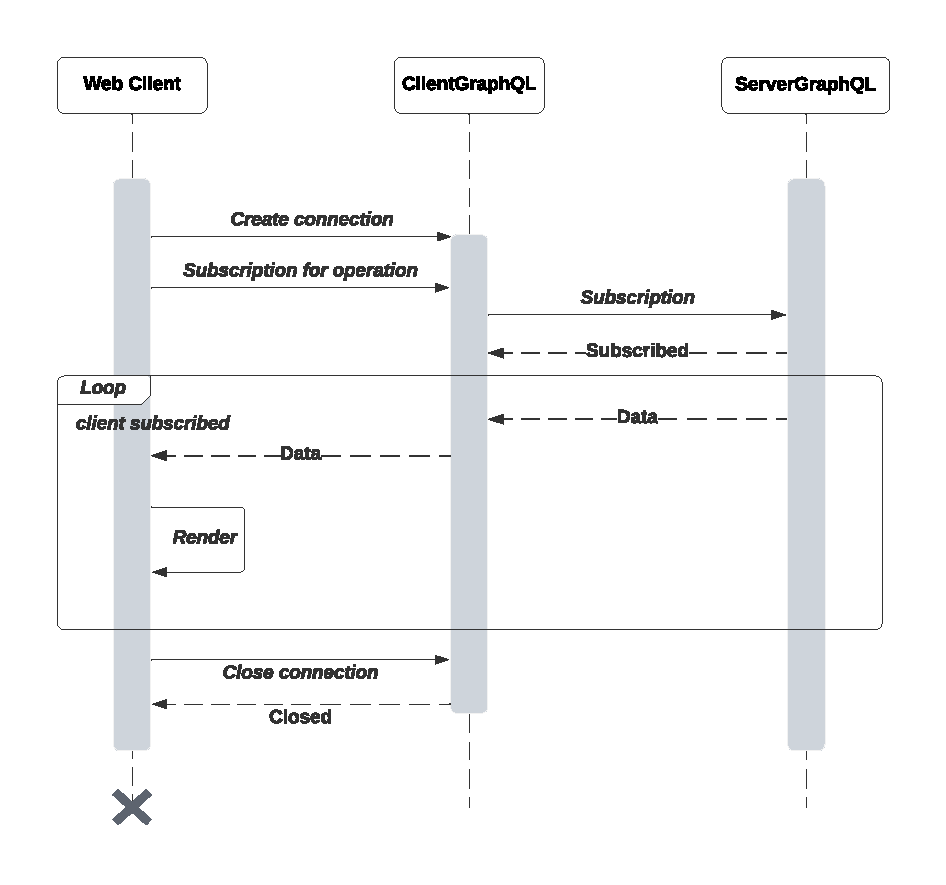
\includegraphics[width=.65\linewidth]{imgs/Rendering_Diagramma_Sequenza.pdf}
	\caption{Diagramma di sequenza del rendering dei nodi a seguito di una \textit{subscription}}
	\label{fig:rendering-graphics}
\end{figure}

\subsection{Progetto multiplatform}
\textit{Kotlin Multiplatform}\footnote{\url{https://kotlinlang.org/docs/multiplatform-discover-project.html}} è una tecnologia che permette lo sviluppo di codice Kotlin condivisibile tra diverse piattaforme, come per esempio Android, iOS, web e desktop. Questo significa che è possibile utilizzare lo stesso codice Kotlin per creare applicazioni native per diverse piattaforme, riducendo la necessità di scrivere e mantenere implementazioni separate per ciascuna piattaforma.
Caratteristica dei progetti multipiattaforma è che sono composti dai cosiddetti \textit{source sets}: insiemi di codice sorgente specifici alla piattaforma a cui si riferiscono. Generalmente è sempre presente il modulo comune, detto ``common code''. Questo modulo contiene il codice condiviso che può essere utilizzato su tutte le piattaforme. Ad accompagnarlo quindi sono altri \textit{source sets} aggiuntivi, compilati per target diversi come \ac{JVM}, JavaScript o nativo.  
Al momento della compilazione di un progetto multi-piattaforma per un target specifico, Kotlin raccoglie tutti i \textit{source sets} contrassegnati con quel target e produce da essi i file binari (come file \textit{.jar} per JVM, file \textit{.js} per JavaScript, ecc.) che possono essere utilizzati nell'ambiente di destinazione corrispondente.
Questo approccio consente una maggiore flessibilità e compatibilità nella creazione di applicazioni multi-piattaforma utilizzando Kotlin.
\begin{figure}
	\centering
	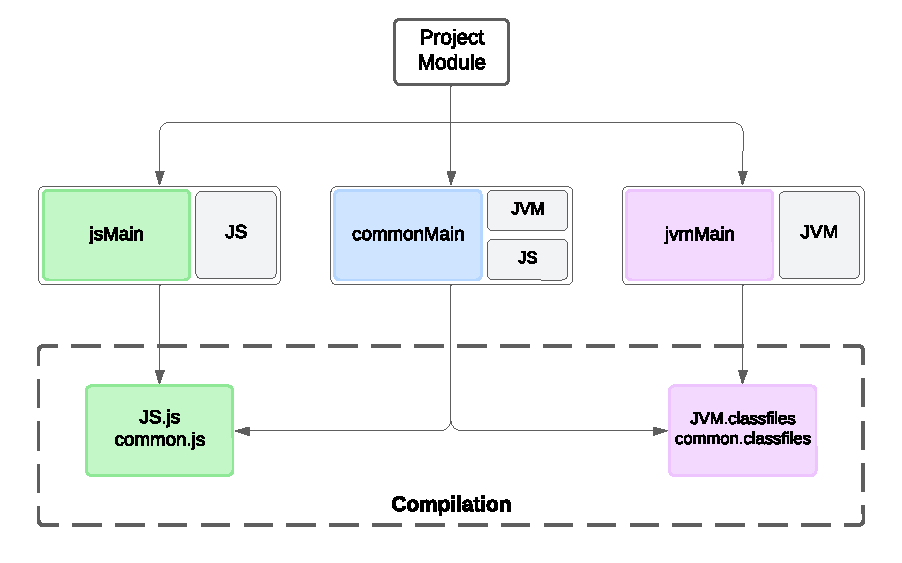
\includegraphics[width=.7\linewidth]{imgs/MPProject.pdf}
	\caption{Struttura di un progetto multipiattaforma compilato per KotlinJS e KotlinJVM}
	\label{fig:mpp-project}
\end{figure}
Nel caso dello sviluppo di una applicazione in-browser il progetto potrebbe includere i seguenti \textit{source sets}:
\begin{itemize}
	\item \textbf{Common Source Set}: Codice condiviso che può essere utilizzato su tutte le piattaforme target. 
	\item \textbf{JVM Source Set}: Codice destinato al target \ac{JVM}. Da qui può essere gestita una componente server dal quale sarà accessibile l'interfaccia grafica.
	\item \textbf{JavaScript Source Set}: insieme di file sorgente destinato al target JavaScript. Il codice scritto in linguaggio Kotlin viene compilato per il target JavaScript (da qui la denominazione KotlinJS). In questo sottomodulo viene definita la struttura e il comportamento dell'interfaccia grafica vera e propria.
\end{itemize}

\section{Analisi e Modello del Dominio}
Uno dei requisti di questo applicativo verte sul bisogno di creare una piattaforma web tale da impiegare le \ac{API} esposte dall'infrastruttura GraphQL fornita. Pertanto, non esiste una comunicazione diretta tra il client web e la simulazione di Alchemist. La gestione dell'accesso e del recupero dei dati dal modello della simulazione è affidata alla componente server, che, al contempo, fornisce anche un punto di accesso ai client che richiedono tali dati~\cite{amslaurea30280}.
Il client web quindi comprende un modulo (nella \cref{fig:domain-model} \texttt{GraphQLClient}) che si pone da interfaccia tra l'applicazione web vera e propria e l'\textit{endpoint} sulla quale la componente server utilizzerà per ricevere richieste e mandare risposte (\textit{endpoint} \texttt{/graphql}). 
Il compito del client web quindi sarà quello di utilizzare le operazioni possibili (\textit{query}, \textit{mutation} e \textit{subscription}) e recuperare i risultati per rappresentarli graficamente. In una prospettiva generale, il ruolo ricoperto dal client web sarà quello di \textit{View} nel pattern architetturale \textit{ \ac{MVC}}~\cite{Gamma1994}.

Alchemist presenta già altri moduli che raffigurano l'ambiente di simulazione, implementati con tecnologie differenti a quelle che verranno proposte successivamente in questo elaborato. Il modulo specifico che viene avviato per rappresentare la simulazione dipende dalla configurazione con cui viene avviato l'intero software. Di conseguenza, è opportuno che l'interfaccia web e la componente server vengano avviate esclusivamente attraverso una specifica configurazione della simulazione.

\begin{figure}[htb]
	\centering
	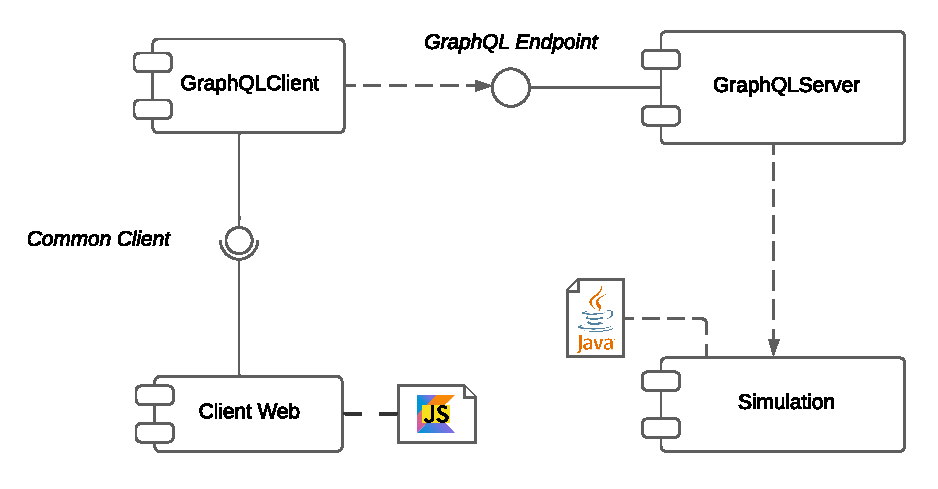
\includegraphics[width=.8\linewidth]{imgs/domain_model.pdf}
	\caption{Diagramma UML dei componenti dell’architettura di alto livello}
	\label{fig:domain-model}
\end{figure}



